\documentclass[aps,prl,twocolumn,10pt,superscriptaddress]{revtex4-1}
% \documentclass[aps,twocolumn,secnumarabic,balancelastpage,amsmath,amssymb,nofootinbib]{revtex4-1}
\usepackage{amsmath}
\usepackage{amssymb}
\usepackage{amsfonts}
\usepackage{color}
\usepackage{graphics}
\usepackage[pdftex]{graphicx}
\usepackage[utf8x]{inputenc}
\usepackage[colorlinks=true]{hyperref}
\usepackage{footmisc}
\usepackage{braket}

\newcommand{\ud}{\mathrm{d}}
\newcommand{\ue}{\mathrm{e}}
\newcommand{\ui}{\mathrm{i}}
\newcommand{\res}{\mathrm{Res}}
\newcommand{\Tr}{\mathrm{Tr}}
\newcommand{\dsum}{\displaystyle\sum}
\newcommand{\dprod}{\displaystyle\prod}
\newcommand{\dlim}{\displaystyle\lim}
\newcommand{\dint}{\displaystyle\int}
\newcommand{\fsno}[1]{{\!\not\!{#1}}}
\newcommand{\texp}[2]{\ensuremath{{#1}\times10^{#2}}}
\newcommand{\dexp}[2]{\ensuremath{{#1}\cdot10^{#2}}}
\newcommand{\eval}[2]{{\left.{#1}\right|_{#2}}}
\newcommand{\paren}[1]{{\left({#1}\right)}}
\newcommand{\lparen}[1]{{\left({#1}\right.}}
\newcommand{\rparen}[1]{{\left.{#1}\right)}}
\newcommand{\abs}[1]{{\left|{#1}\right|}}
\newcommand{\sqr}[1]{{\left[{#1}\right]}}
\newcommand{\crly}[1]{{\left\{{#1}\right\}}}
\newcommand{\angl}[1]{{\left\langle{#1}\right\rangle}}
\newcommand{\tpdiff}[4][{}]{{\paren{\frac{\partial^{#1} {#2}}{\partial {#3}{}^{#1}}}_{#4}}}
\newcommand{\tpsdiff}[4][{}]{{\paren{\frac{\partial^{#1}}{\partial {#3}{}^{#1}}{#2}}_{#4}}}
\newcommand{\pdiff}[3][{}]{{\frac{\partial^{#1} {#2}}{\partial {#3}{}^{#1}}}}
\newcommand{\diff}[3][{}]{{\frac{\ud^{#1} {#2}}{\ud {#3}{}^{#1}}}}
\newcommand{\psdiff}[3][{}]{{\frac{\partial^{#1}}{\partial {#3}{}^{#1}} {#2}}}
\newcommand{\sdiff}[3][{}]{{\frac{\ud^{#1}}{\ud {#3}{}^{#1}} {#2}}}
\newcommand{\tpddiff}[4][{}]{{\left(\dfrac{\partial^{#1} {#2}}{\partial {#3}{}^{#1}}\right)_{#4}}}
\newcommand{\tpsddiff}[4][{}]{{\paren{\dfrac{\partial^{#1}}{\partial {#3}{}^{#1}}{#2}}_{#4}}}
\newcommand{\pddiff}[3][{}]{{\dfrac{\partial^{#1} {#2}}{\partial {#3}{}^{#1}}}}
\newcommand{\ddiff}[3][{}]{{\dfrac{\ud^{#1} {#2}}{\ud {#3}{}^{#1}}}}
\newcommand{\psddiff}[3][{}]{{\frac{\partial^{#1}}{\partial{}^{#1} {#3}} {#2}}}
\newcommand{\sddiff}[3][{}]{{\frac{\ud^{#1}}{\ud {#3}{}^{#1}} {#2}}}
\newcommand{\eff}{ef\! f}
\newcommand{\Na}{\mathrm{Na}}
\newcommand{\Cs}{\mathrm{Cs}}
\newcommand{\fxnote}[1]{{\textbf{[#1]}}}

\newcommand{\todo}[1]{}

\ifpdf
% Ensure reproducible output
\pdfinfoomitdate=1
\pdfsuppressptexinfo=-1
\pdftrailerid{}
\hypersetup{
  pdfcreator={},
  pdfproducer={}
}
\fi

\newcommand{\harvardphysics}{\affiliation{Department of Physics, Harvard University, Cambridge, Massachusetts 02138, USA}}
\newcommand{\harvardccb}{\affiliation{Department of Chemistry and Chemical Biology, Harvard University, Cambridge, Massachusetts 02138, USA}}
\newcommand{\cua}{\affiliation{Harvard-MIT Center for Ultracold Atoms, Cambridge, Massachusetts 02138, USA}}
\newcommand{\gradstudent}{
  \harvardphysics
  \harvardccb
  \cua
}

\begin{document}
% \title{Coherent optical association of atoms into a single molecule}
\title{Coherent optical creation of a single molecule}
\author{Yichao~Yu}
\email{yichaoyu@g.harvard.edu}
\gradstudent
\author{Kenneth~Wang}
\gradstudent
\author{Jonathan~D.~Hood}
\affiliation{Department of Chemistry, Purdue University, West Lafayette, Indianna, 47906, USA}
\author{Lewis~R.~B.~Picard}
\gradstudent
\author{Jessie~T.~Zhang}
\gradstudent
\author{William~B.~Cairncross}
\harvardccb
\harvardphysics
\cua
\author{Jeremy~M.~Hutson}
\affiliation{Joint Quantum Centre Durham-Newcastle, Department of Chemistry, Durham University, Durham, DH1 3LE, United Kingdom}
\author{Till Rosenband}
\harvardphysics
\author{Kang-Kuen~Ni}
\email{ni@chemistry.harvard.edu}
\harvardccb
\harvardphysics
\cua

\date{\today}

\begin{abstract}
  We report on coherent association
  of atoms into a single weakly bound NaCs molecule in an optical tweezer
  through an optical Raman transition.
  The Raman scheme uses a deeply bound electronic excited intermediate state
  to achieve a large transition dipole moment while reducing photon scattering.
  Starting from two atoms in their relative motional ground state,
  we achieve an optical transfer efficiency of $69\mathrm{\%}$.
  The molecules have a binding energy of $770.1969(2)~\mathrm{MHz}$ at $8.83(2)~\mathrm{G}$
  and are created with higher than $60\mathrm{\%}$ probability in the motional ground state.
  This technique does not rely on Feshbach resonances or narrow excited-state lines
  and may allow a wide range of molecular species to be assembled atom-by-atom.
\end{abstract}

\maketitle

% Introduction


% 1. we want to have a diverse species to tailor to different applications including precision measurements and quantum engineering. 2. for the technique of associating atoms to form molecules, but so far all has been done with Feshbach association (before STIRAP), or in the case of Sr2, a narrow excited state. Previous work on near-threshold Raman transfer has been incoherent.
% (suggested referees: Florian Shreck and Immanual Bloch, Tanya, Deep Gupta, DeMille)

% Trapped neutral molecules, assembled in an array of optical tweezers, are a promising platform to study quantum information and quantum simulation. (more detail to add here about applications?).

Diverse species of fully quantum controlled  ultracold molecules are desired
for a wide variety of applications including precision measurements~\cite{
  Kondov2019,Nick_and_Ivan2017, PhysRevA.101.042504, Andreev2018,
  PhysRevLett.119.153001, hudson2011},
quantum simulations~\cite{Micheli2006, Yao2018, Wall2015, wall2015realizing},
quantum information processing~\cite{DeMille2002, Ni2018, Hudson2018, Lin2019},
and studies of ultracold chemistry~\cite{Bala2016,Hu1111,Segev2019,deJongh626}.
While many innovative approaches demonstrated in the last few years
have directly cooled different species of diatomic or polyatomic molecules
below 1~mK~\cite{Norrgard2016,Anderegg2018, Mitra1366, PhysRevX.10.021049,
  PhysRevLett.121.013202, Truppe2017},
the highest phase-space-density gas~\cite{Demarco2018} and
the coldest individual molecules~\cite{Zhang2020,He331}
have been achieved through the association of ultracold atoms.
% (any place to cite molecular ion work?)
% Citations are not complete. Add them as you see fit.

Molecular association of ultracold atoms takes advantage of the cooling and trapping techniques
that have been developed for atoms.
Associating atoms into deeply bound molecules is challenging
because of the small wavefunction overlap between the free-atom and molecular states
and the release of a large amount of binding energy.
A widely used method of overcoming these challenges is to associate atom pairs
into weakly bound molecules first,
and then transfer the molecules from this single internal state
to a desired rovibrational and electronic state,
releasing the binding energy by stimulated emission~\cite{Danzl2008, Ni2008, Lang2008,
  Takekoshi2014, Molony2014, Park2015, Guo2016, Kondov2019, Voges2020}.
So far, molecular association has generally been achieved by magnetoassociation
using a magnetic Feshbach scattering resonance.
Exceptions include Sr$_2$, where narrow linewidth ($\sim 20~\mathrm{kHz}$) excited states
are available and optical association can be driven coherently~\cite{Reinaudi2012,Stellmer2012},
and $^{87}$Rb$^{85}$Rb,
where there are molecular states bound by $1-2~\mathrm{MHz}$~\cite{He331}.
With these requirements, molecules involving non-magnetic atoms
or atoms without narrow intercombination lines remain difficult to associate.
% These requirements limit the generality of previous association techniques.
% The requirement of a Feshbach resonance or a MHz-level binding energy bound state to enhance atom-to-molecule wavefunction overlap or the existence of narrow excited-state lines limits the generality of previous association techniques. % to more diverse species.



Here, we demonstrate coherent association of an atom pair to a weakly bound molecule
by two-photon optical Raman transfer via an electronic excited state,
schematically shown in Fig.~\ref{f-theory}a.
The scheme does not rely on a Feshbach resonance,
molecular states bound by a few MHz, or a narrow excited state.
The resulting single molecule is in a well-defined internal quantum state
and predominantly in its motional ground state.
A vibrational state of the electronic excited state $\mathrm{c^3\Sigma^+}(\Omega = 1)$
is used as the intermediate state in the Raman scheme,
and is chosen to minimize photon scattering during Raman Rabi oscillations.
To reduce photon scattering and sensitivity to laser intensity noise further,
we choose the initial and final states to balance the two Rabi frequencies as much as possible.
This system-independent approach creates molecules atom-by-atom with full quantum state control.


\begin{figure*}
  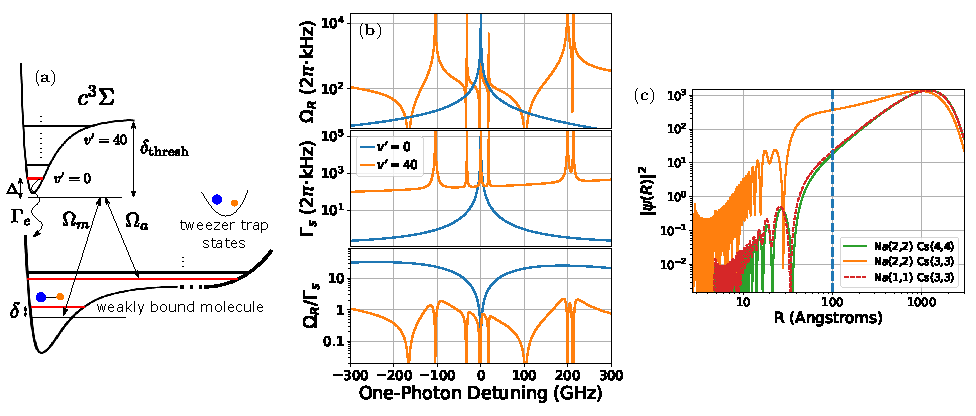
\includegraphics[width=\textwidth]{imgs/fig-theory.pdf}
  \caption{Optical creation of single molecule from single atoms in tweezer.
    (a) Schematic of the optical transition from an atom pair to a weakly bound molecule.
    The initial state is the relative motional ground state between the two atoms
    and the final state is the first molecular bound state.
    The transition is driven by a pair of laser frequencies matching the binding energy
    of the molecule.
    The lasers are detuned from an excited molecular state in the $\mathrm{c^3\Sigma}$ potential
    by $\Delta$ in order to suppress scattering during the transfer.
    (b) Comparison between using a weakly bound and a deeply bound excited state
    as intermediate state for the Raman transition.
    The deeply bound excited state (blue lines $v'=0$)
    has a smaller Raman Rabi frequency ($\Omega_{R}$)
    compared to the weakly bound excited state (orange lines $v'=40$) at a most detuning.
    However, the scattering rate ($\Gamma_{s}$) is also much lower,
    which results in a larger ratio of Raman Rabi frequency to scattering rate.
    (c) Enhancement of the short-range wavefunction.
    The large scattering length for the $\Na(2,2),\Cs(3,3)$ state creates an interaction shift
    comparable to the axial trapping frequency.
    This causes a significant change in the relative wavefunction, especially at short
    internuclear distance ($R$).
    Compared to other spin states with weaker interaction,
    the wavefunction at short distance ($R<100\ \text{\AA}$, left of the dashed line)
    is significantly enhanced.
    \label{f-theory}
  }
\end{figure*}

\begin{figure}
  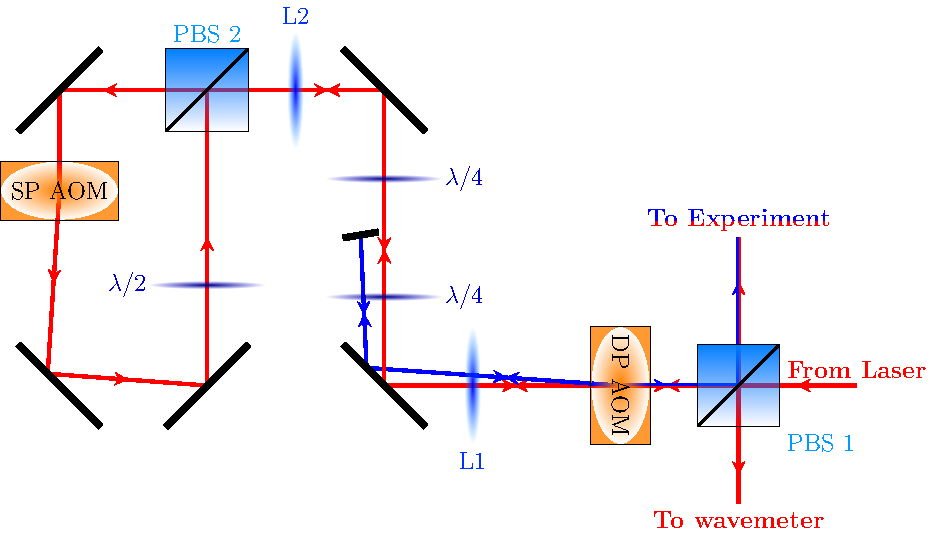
\includegraphics[width=0.5\textwidth]{imgs/raman_spectroscopy_raman_beampath.pdf}
  \caption{
    Beampath for generating the frequency for Raman transition in the tweezer.
    (Some mirrors and other optics used for alignment are not included.)
    The two ASE filters before and after the fibers are also shown.
    The red beam path is the $0$-th order of the double pass~(DP) AOM
    which is used for the tweezer.
    When the double-pass~(DP) AOM is turned on, some power is redirected to the first order
    (blue beam path) which generates the required frequency different to drive
    the Raman transition. The two frequencies are recombined on the DP AOM.
    The $0$-th order light is shifted by another single pass~(SP) AOM
    running on a different frequency before recombining.
    Without this AOM, the leak light from the DP AOM will be at the same frequency
    as the $0$-th order light which can cause a significant power fluctuation
    due to interference.
    The experiment typically start with the SP AOM on and the DP AOM off.
    When driving the Raman transition, the powers on both AOMs are ramped simultaneously
    to achieve the desired power at both frequencies.
    \label{f-beampath}
  }
\end{figure}


The essence of an optical Raman transfer can be illustrated
using a three-level system shown in Fig.~\ref{f-theory}a,
where the initial atomic state and the target weakly bound molecular state are coupled to an intermediate state by two lasers with Rabi frequencies, $\Omega_a$ and $\Omega_m$, with one-photon detuning $ \Delta $, and two-photon detuning, $ \delta$.  %(Ultimately, we calculate with contribution of all vibrational states of the excited electronic potential, $\mathrm{c^3\Sigma^+}$)
The transfer Raman Rabi Rate is given by $\Omega_a\Omega_m / 2\Delta$~\cite{Wineland2003}.
% , is accompanied by a photon scattering rate $\Gamma_e (\Omega_a^2 + \Omega_m^2)/4\Delta^2$
% $\Gamma_e \Omega^2 / 4\Delta^2 $, where $ \Gamma_e $ is the excited state linewidth
Unlike Raman transitions in atoms, the two Rabi frequencies are greatly imbalanced %. Since $ \Omega_m $ is generally much larger than $ \Omega_a $
due to the small wavefunction overlap between the atomic state and the intermediate state, %the atomic state and the excited molecular state,
and therefore the scattering is predominantly from the target molecular state. Furthermore, the energy difference between the atomic state and target molecular state is small ($ < 1~\mathrm{GHz} $) compared to the single-photon detuning, $ \Delta $, so the target molecular state can scatter off both beams roughly equally. Thus, the scattering rate is given by $ \Gamma_e \Omega_m^2 / 2\Delta^2$, where $ \Gamma_e $ is the excited-state linewidth \footnote{We choose the two beams to have equal power, which gives the highest Raman Rabi rate at a fixed total power. Thus, this results in a simple factor of 2 coming from scattering off 2 beams.}.
The ratio between the Raman Rabi frequency and the scattering rate is therefore $ \Omega_a/\Omega_m \times \Delta/\Gamma_e $. %, depends on the ratio of the two matrix elements and how far detuned the laser is from the transition in units of the linewidth.
To ensure a coherent process, a detuning as large as possible, while maintaining a realistic Raman Rabi frequency, is preferred. %However, the detuning cannot be too large, since that will reduce the Raman Rabi frequency.

Earlier experiments used weakly bound excited states as the intermediate state
in the Raman transition to ensure a large Raman Rabi frequency~\cite{Wynar2000,Rom2004}.
However, a complete picture must include both the many vibrational levels
of the excited electronic state and the atomic continuum.
The total scattering rate and Raman Rabi rate become a sum of the scattering rates
and Raman Rabi rates over all possible intermediate states.
Since there is large overlap between the target molecular state and weakly bound excited states, using states that are closer to the dissociation threshold as the intermediate state results in a large scattering rate.
% in large incoherence and loss to other molecular states.
This scattering is approximately proportional to $1/\delta_{\mathrm{thresh}}^2$,
where $\delta_{\mathrm{thresh}}$ is the detuning from the dissociation threshold,
and thus can be made smaller by using deeply bound vibrational states as the intermediate state.


To find the optimal intermediate state, we perform a calculation of the Raman Rabi frequency $\Omega_R$
and scattering rate $\Gamma_s$ at different detunings from the atomic threshold
taking into account of all states of
8 excited molecular potentials~\cite{Korek2007, Grochola2011, Zaharova2009, Grochola2010, Zabawa2012}
and the continuum~\cite{Liu2017}.
This calculation shows that $\Omega_R/\Gamma_s$
can be made larger for more deeply bound states compared to weakly bound states
at a cost of a smaller $\Omega_R$, as shown in Fig.~\ref{f-theory}b;
see Supplementary Material for details.
As a result, we choose the $v'=0$ level of $\mathrm{c^3\Sigma^+}(\Omega = 1)$
as the closest intermediate state to drive the Raman transition.

In addition to the intermediate state,
choosing an initial and a final state for a large ratio $\Omega_a/\Omega_m$
maximizes $\Omega_R$ at a given detuning.
Furthermore, a larger ratio also relaxes the intensity stability requirement for the Raman lasers,
because this is also the ratio between $\Omega_R$
and the AC Stark shift of the molecular state, $\Omega_m^2 / 2\Delta$
\footnote{There is an additional factor of 2, with both beams at equal power,
  to account for the Stark shift caused by both beams.}.
Due to the small extent of the intermediate-state wavefunction
compared to that of the trapped atoms,
$\Omega_a$ is approximately proportional to
the amplitude of the relative atomic wavefunction at short distance,
within the range of the molecular potential.
To increase this amplitude, one can increase the external confinement of atom pairs.
Using a harmonic approximation,
the short-range amplitude is proportional to $ \omega_{\text{trap}}^{3/4} $ or $P^{3/8}$,
where $ \omega_{\text{trap}} $ is the trap frequency and $P$ is the optical power in the tweezer trap \cite{Mies2000}. However, additional power may not always be available, and will also lead to additional undesired scattering.
Alternatively, one can choose an atomic pair state with a large scattering length
(positive or negative).
For such states, the amplitude of the relative atomic wavefunction is substantially enhanced
at short range, as shown in Fig.~\ref{f-theory}c.
% The increase in the coupling is proportional to (quote/cite Olive's equation?).
For our system of Na and Cs atoms,
we choose a spin-state combination $\ket{\uparrow_{\Na} \downarrow_{\Cs}}\equiv \ket{f=2,m_f=2}_{\Na}\ket{f=3,m_f=3}_{\Cs}$ that has a large and negative scattering length of
$a(\uparrow_{\Na} \downarrow_{\Cs}) \approx -700a_0$~\cite{Hood2019}.
All other stable spin combinations give smaller scattering lengths ($<~50~a_0$).
% We denote the possible hyperfine states of the atoms as $ \ket{\uparrow_{\Cs}} = \ket{f=4,m_f=4}_{\Cs}, \ket{\downarrow_{\Cs}} = \ket{f=3,m_f=3}_{\Cs}, \ket{\uparrow_{\Na}} = \ket{f=2,m_f=2}_{\Na}, $ and $ \ket{\downarrow_{\Na}} = \ket{f=1,m_f=1}_{\Na}$. Among the stable spin combinations, $\ket{\uparrow_{\Na}\uparrow_{\Cs}}$ and $\ket{\downarrow_{\Na}\downarrow_{\Cs}} $ both have small scattering lengths of $ 30.4a_0 $, and $ 13.7a_0 $ respectively, but the $\ket{\uparrow_{\Na} \downarrow_{\Cs}} $ combination has a large and negative scattering length of $ a(\uparrow_{\Na} \downarrow_{\Cs}) = -693.8a_0 $ (interaction shift $\approx$ binding?)~\cite{Hood2019}.

To identify a suitable target molecular state, we carry out coupled-channel calculations of the near-threshold bound states, as described in the Supplemental Material.
Choosing a bound state with similar spin character to the atomic state  minimizes the sensitivity of the transition frequency to magnetic field.
A suitable state with this character is predicted about 763 MHz below the $\ket{\uparrow_{\Na} \downarrow_{\Cs}}$ threshold.
% The coupled-channel calculations show that this target molecular state has lower overlap with the intermediate state, compared to bound states from other hyperfine combinations.
% For the target molecular state, the spin state is ideally similar to the initial spin state in order to minimize sensitivity to the magnetic field.
% We find a target spin state predominantly in the initial spin state
% that also has the advantage of having a reduced sensitivity
% to laser intensity noise because of a larger %$\Omega_a/\Omega_b$ as compared to other states.
% This reduces the intensity stability requirement to $5~\mathrm{\%}$
% instead of $0.3~\mathrm{\%}$ which is typical for other states.
% In addition to the increased atomic coupling, $ \Omega_a $,
% Coupled-channel calculations show that this target molecular state with similar spin composition also has reduced Rabi frequency, $ \Omega_m $, with the intermediate state when compared to bound states of the other spin compositions.
The ratio $\Omega_a/\Omega_m$ increases to about 0.013 when starting from atoms in the $\ket{\uparrow_{\Na} \downarrow_{\Cs}}$ hyperfine combination.
% $\ket{\uparrow_{\Na}\uparrow_{\Cs}}$ and $\ket{\downarrow_{\Na}\downarrow_{\Cs}} $ bound states.
Compared to 0.003
with the other combinations, this relaxes the intensity stability requirement to the percent level. % Thus, instead of a required intensity stability of $0.3 ~\mathrm{\%} $ for the 4422 or 3311 combination, the 3322 combination only requires the intensity to be stabilized to $ 5~\mathrm{\%} $.
% Thus, we choose the $\ket{\uparrow_{\Na} \downarrow_{\Cs}}$ spin combination as our initial state and drive to the first bound state for the $\ket{\uparrow_{\Na} \downarrow_{\Cs}}$ spin combination.
% \textcolor{blue}{(clean up the paragraph some more).} %(We might want to mention that those ratios are for 80 kHz spherical trap if we want to give more details about the coupled-channel calculation anywhere...)

% In additional to the final and the excited state, it is also important to select the an initial atomic state in order to improve the coupling.
\begin{figure}[ht!]
  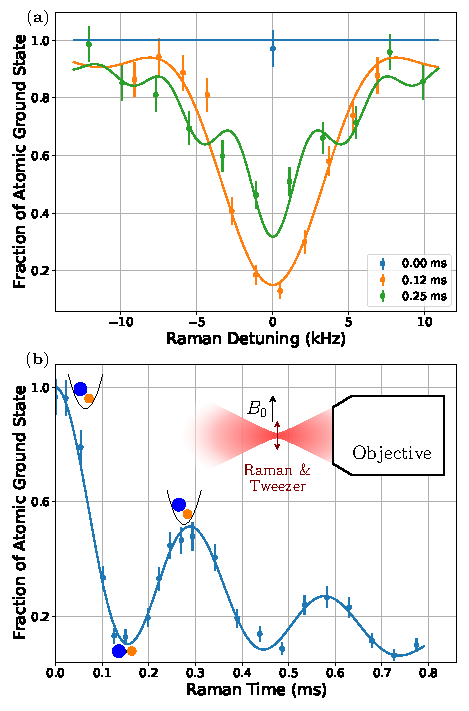
\includegraphics[width=0.48\textwidth]{imgs/fig-raman.pdf}
  \caption{
    (a) Raman detuning scans at different times showing the resonance frequency.
    (b) Raman pulse-time scan on resonance.
    A decaying Rabi oscillation can be observed, proving the coherence of
    the Raman transfer process.
    This is fitted together with (a) to a model of the Raman transition including loss of the atom and molecule state and is used to determine
    both the Raman Rabi frequency and the loss rates.
    Inset: Geometry and polarization of trap and Raman beam relative to the bias magnetic field.
    The tweezer and Raman beam is focused through an objective to a waist of $0.9~\mathrm{\mu m}$,
    which defines the location of the atoms and molecule.
    We use a bias magnetic field $B_0=8.83(2)~\mathrm{G}$ along the tweezer polarization
    to define the quantization axis.
    As a result, the atoms experience predominantly $\pi$ polarization from the tweezer.
    \label{f-raman}}
\end{figure}

%% Preparation
Experimentally, we first prepare two atoms in a well-defined external and internal quantum state
using techniques developed previously~\cite{Liu2018, Liu2019, Wang2019}.
In brief, the experimental cycle begins by stochastically loading a single ${}^{23}\Na$ atom
and a single ${}^{133}\Cs$ atom into separate optical tweezers.
The atoms are initially imaged to distinguish between loading of two atoms,
one atom (Na or Cs), or no atom to be able to post-select from the experimental results
based on the initial loading condition.
After imaging, we turn on a $8.83(2)~\mathrm{G}$ magnetic field to define the quantization axis
for the state preparation and molecule formation steps.
Raman sideband cooling is then applied to prepare both atoms simultaneously
in the 3-dimensional motional ground state of their optical tweezers.
After cooling, the Na and Cs atoms are in the spin state~$\ket{\uparrow_{\Na}\uparrow_{\Cs}}\equiv \ket{f=2,m_f=2}_{\Na}\ket{f=4,m_f=4}_{\Cs}$,
which has a small scattering length.
The weak two-atom interaction allows the merging of the two tweezers to be done
with minimum pertubation so that they remain in the motional ground state.

% After preparing the Na and Cs atoms in the same tweezer in a single quantum state,
Next, we drive the atoms into spin combination $\ket{\uparrow_{\Na} \downarrow_{\Cs}}$,
which has large scattering length,
by performing a Cs spin flip while taking into account
the $-30.7~\mathrm{kHz}$ interaction shift~\cite{Hood2019}.
We use this as the initial atomic state for Raman transfer.
This spin flip selectively transfers atoms in the relative motional ground state,
removing any background from atoms in excited motional states
\footnote{This interaction shift is larger than the differential axial trapping frequency
  between Na and Cs atoms, which decouples the relative and center of mass motional state
  and improves the robustness of our preparation of the relative motional ground state.}.
For the experiment reported here,
$31\mathrm{\%}$ of our initial two-atom population is transferred.
% of two atoms loaded in separate optical tweezers.\textcolor{red}{I also find this part of the sentence confusing.  can you say this more concisely?}\todo{}
% The stronger interaction in this spin state also enhances the atomic wavefunction at short range and increases its overlap with the intermediate molecular state used for our Raman transfer..

%% Transfer scheme
% After the atoms are prepared in the $\ket{\uparrow_{\Na}\uparrow_{\Cs}} $ hyperfine combination, we then perform the Raman transfer.
To perform the Raman transfer of an atom pair to the target weakly bound molecular state,
we use the tweezer beam itself as the Raman beams by turning on two frequencies
in the tweezer during the Raman pulse using an acousto-optic modulator, as shown in Fig.~\ref{f-beampath}.
The dual use of the tweezer beam not only eliminates additional scattering sources
or undesired laser frequencies,
but also allows a tight focus to maximize the Raman Rabi frequency
and minimize the transfer time.
Furthermore, we use two Bragg gratings, each with a linewidth (FWHM) of $50~\mathrm{GHz}$,
to filter the laser spectrum.
As shown in Fig.~\ref{f-beampath}, we place one filter directly after the laser, which is a fiber amplifer seeded with a $1037~\mathrm{nm}$ external cavity diode laser. We place the second filter as close to the microscope objective as possible.
We observe a reduction of the scattering rate by a factor of $2$
due to suppression of the broadband amplified spontaneous emission (ASE) from the laser
that couples to other excited states.
After the total tweezer power is set to the desired value,
we smoothly ramp down the power of one frequency in the tweezer
while simultaneously ramping up the power of the other frequency
so that the total tweezer power remains unchanged.
Both frequencies are kept on for a specified duration before the process is reversed
and the tweezer returns to a single frequency.

% found the spectral purity of the laser for Raman beams to be critical for achieving a higher transfer efficiency.
% The tweezer/Raman beams are generated by a fiber amplifier seeded with a $1037~\mathrm{nm}$ external cavity diode laser.
% by amplifying a $1037~\mathrm{nm}$ external cavity diode laser (ECDL) with a fiber amplifier,
% The diode laser produces the desired frequency on top of a broad band amplified spontaneous emission (ASE).  We use a Bragg grating with a line width (FWHM) of $50~\mathrm{GHz}$ to clean up the laser spectrum and found it reduces the scattering rate by at least a factor of $2$
% for a particular single-photon detuning.

% in addition to the desired frequency. This increases the scattering rate due to coupling to other excited states.



%% Experiment condition/resonance

\begin{figure}[t!]
  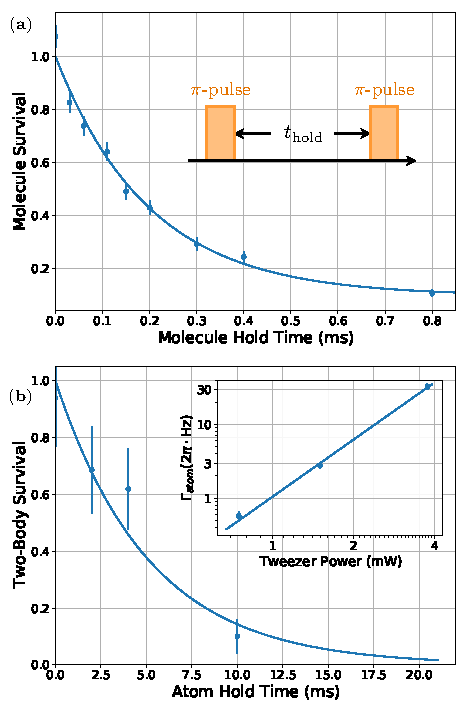
\includegraphics[width=0.48\textwidth]{imgs/fig-lifetime.pdf}
  \caption{
    (a) Direct measurement of molecule lifetime in a trap of depth $3.75~\mathrm{mW}$.
    Molecule survival is detected by dissociating back to atoms using a second Raman transition.
    The lifetime is consistent with the $0.199(9)~\mathrm{ms}$
    measured from the Raman transition data.
    Inset: pulse sequence for the lifetime measurement.
    (b) Two-body atom lifetime of $5(1)~\mathrm{ms}$
    in a trap of depth $3.75~\mathrm{mW}$ caused by off-resonance photoassociation.
    This is used to improve the fitting of the Raman transfer data.
    Inset: Atomic scattering rate scales as
    $P_\textrm{tweezer}^{2.58}\times\!2\pi\!\times29.3(17)~\mathrm{mHz/mW^{2.58}}$ on a log-log scale;
    this is consistent with a two-photon scattering process.
    We have not measured a clear dependency of the loss rate on the tweezer detuning.
    \label{f-lifetime}}
\end{figure}

We choose the tweezer frequency to be $288560~\mathrm{GHz}$
which is far detuned (by $\approx\!151~\mathrm{GHz}$) from the $v' = 0$ line.
Guided by the coupled-channel calculations,
we locate the Raman resonance for the atoms-to-molecule transition at
$770.57150(9) ~\mathrm{MHz}$ with about $3.75~\mathrm{mW}$ tweezer power
focused down to a waist of $ 0.9~\mathrm{\mu m}$, as shown in Fig.~\ref{f-raman}a.
% (We can maybe add information about the prediction here?)
%% Prediction
% This excited state used in the Raman transition was measured in our previous experiment using photoassociation to be at $288560 GHz$ from our atomic state. The ground molecular state has not been observed previously in experimentally. Based on our measurement of FB resonance, interaction shift and the binding energy of the 4422 bound state. Theory prediction was at $770.1 MHz$.
% The background level of $31~\mathrm{\%}$ corresponds to the probability of preparing the two atoms in the relative motional ground state.
% When the atoms are transferred into the molecule state by the Raman transition, there is a decrease in the two body survival since the resulting molecule is dark to our imaging sequence. % directly detected by our imaging step.
The molecular state is dark to the imaging step,
so successful transfer of the atoms to the molecular state is detected as loss of atoms.
We observe a Fourier-limited linewidth, which is evidence of a coherent transfer.
In order to verify the coherence of the transfer directly,
we fix the two-photon detuning on resonance and scan the pulse time.
Fig.~\ref{f-raman}b shows the observed coherent Rabi oscillation between the atomic and molecular states.
Fitting the data with a decaying Rabi oscillation suggests that
$69~\mathrm{\%}$ of atoms initially in the motional ground state are transferred into the molecular state after a $\pi$ pulse.
This transfer efficiency is limited mainly by the molecular lifetime,
which can be measured directly by preparing the molecule with a $\pi $ pulse
and then using a second $\pi$ pulse to dissociate the molecule back to atoms
after a variable wait time.
The result in Fig.~\ref{f-lifetime}a shows a molecular lifetime of $0.199(9)~\mathrm{ms}$
consistent with the decay of the Rabi oscillation.
We obtain the Raman Rabi frequency by fitting our measurements to a model
that includes a Raman Rabi frequency and
a finite lifetime for the molecular state, as shown in Fig.~\ref{f-raman}a and b.
We account for the small effect of atomic state loss by measuring the one-body and
two-body lifetime of the atoms directly without turning on the second frequency,
as shown in Fig.~\ref{f-lifetime}b.
The fit including all these effects gives a Raman Rabi frequency
of $2\pi\times3.28(4)~\mathrm{kHz}$.

The efficiency of the transfer is lower than expected
because we found the ratio of the molecular scattering rate~(i.e. inverse of lifetime)
to the Rabi frequency is 10 times larger than predicted.
This discrepancy can arise from the $v'=0$ excited state, if the ratio $\Omega_m / \Omega_a$ or $\Gamma_e$ are larger than expected.
Additionally, coupling to other excited states can add an offset to
both the Raman Rabi frequency and the scattering rate and thus affect their ratio.

In order to verify whether any one of these sources are the origin of the reduced transfer efficiency,
we measured the properties of the Raman resonance as a function of the tweezer power and single-photon detuning.
These dependencies allow us to experimentally determine the Rabi frequencies,
$ \Omega_a $, $\Omega_m $ and how much of the scattering, Stark shift,
or Raman Rabi frequency comes from the $ v' = 0$ intermediate state.

\begin{figure*}
  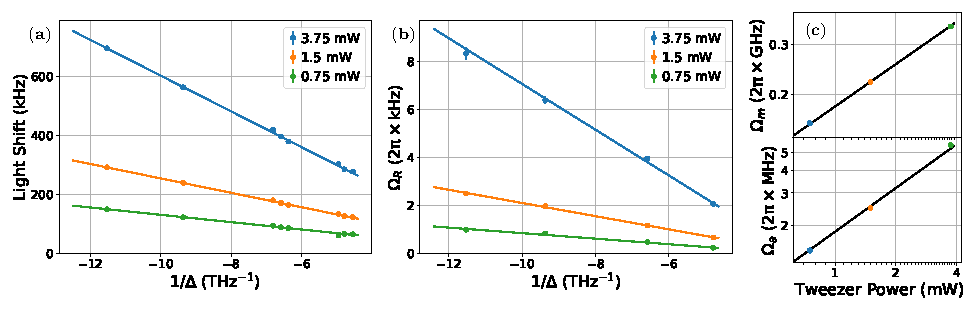
\includegraphics[width=\textwidth]{imgs/fig-det.pdf}
  \caption{Raman transition parameters as a function of tweezer and Raman power and detuning.
    (a) The light shift of the Raman resonance fitted to $a_P+b_P/\Delta$, where
    $a_P$ and $b_P=(\Omega_a^2-\Omega_m^2)/2$
    are tweezer power dependent background and $v'=0$ contribution
    to the light shift,
    $\Delta\equiv f_{\mathrm{PA}0} - f_{\mathrm{tweezer}}$ is the detuning from
    the PA resonance frequency $f_{\mathrm{PA}0}$.
    The $a_P$s are fitted to a model including linear and small quadratic light shift
    \todo{which assumes $\Omega_m\gg\Omega_a$} to obtain the Raman resonance frequency
    at zero tweezer power to be $f_{R0}=770.1969(2)~\mathrm{MHz}$.
    (b) Raman Rabi frequency ($\Omega_R$) fitted to $c_P+d_P/\Delta$, where
    $c_P$ and $d_P=\Omega_a\Omega_m/2$
    are tweezer power dependent background and $v'=0$ contribution.
    The detuning is calculated using the PA frequency fitted in (a).
    The $c_P$s and $d_P$s are proportional to $P^{1.29}$
    and the fit gives $c_P/P^{1.29}=-2\pi\times0.41(2)~\mathrm{kHz/mW^{1.29}}$
    and $d_P/P^{1.29}=-4\pi^2\times167(2)~\mathrm{kHz\cdot GHz/mW^{1.29}}$.
    The fitting results for (a) and (b) are shown in Table~\ref{tab:f-det:fit}.
    (c) Tweezer power dependency of $\Omega_m$ (top) and $\Omega_a$ (bottom) calculated from
    $b_P$ and $d_P$ on a log-log scale showing the $P^{0.5}$ scaling of $\Omega_m$ and
    the $P^{0.79}$ scaling of $\Omega_a$.
    \label{f-det}}
\end{figure*}
\begin{table}[ht]
  \centering
  \begin{tabular}{|c|c|c|c|}
    $P~(\mathrm{mW})$&$0.75$&$1.5$&$3.75$\\\hline
    $f_{\mathrm{PA}0}~(\mathrm{GHz})$&\multicolumn{3}{|c|}{$288711.8$}\\\hline
    $a~(\mathrm{MHz})$&$770.20452(6)$&$770.2081(1)$&$770.1943(3)$\\
    $b~(\mathrm{MHz\cdot GHz})$&$-12.46(2)$&$-24.44(3)$&$-60.66(8)$\\\hline
    $c~(\mathrm{2\pi\times kHz})$&$0.29(2)$&$0.63(4)$&$2.4(2)$\\
    $d~(\mathrm{4\pi^2\times MHz\cdot GHz})$&$0.115(4)$&$0.275(6)$&$0.95(3)$\\
  \end{tabular}
  \caption{Fitting results for Fig.~\ref{f-det}(a,b).
    \label{tab:f-det:fit}}
\end{table}

To determine $\Omega_m$ and $ \Omega_a$, we measure the change in resonance frequency and Raman Rabi frequency as a function of the tweezer detuning.
For both these quantities, we observe a $1/\Delta$ component
and a constant background in the experimentally explored region, as shown in Fig.~\ref{f-det}a, b.
The background is caused by coupling to other excited states that are further away in energy.
The $1/\Delta$ component, however, is due to the coupling to the $v'=0$ intermediate state. Combining the fit coefficients, summarized in Table \ref{tab:f-det:fit}, for the $1/\Delta$ component, we can extract $\Omega_m $ and $ \Omega_a $.

We perform the experiment at various tweezer powers to extract the power dependence of $ \Omega_m $ and $ \Omega_a $, as shown in Fig.~\ref{f-det}c. $ \Omega_m $ scales with $ P^{0.5} $ as expected, and we obtain a fit value of $2\pi\times180.87(7)~\mathrm{MHz}/\sqrt{\mathrm{mW}}$.
This number is within $40~\mathrm{\%}$
of the value $2\pi\times296 ~\mathrm{MHz}/\sqrt{\mathrm{mW}}$ calculated from theory. The scaling of $ \Omega_a $ differs from $ P^{0.5} $, which is the expected scaling from the laser intensity, due to the change in the atomic wavefunction caused by tighter confinement at higher power. For weakly interacting particles,
$\Omega_a$ scales as $P^{3/8}$.
However, due to the strong interaction between the two atoms in the $\ket{\uparrow_{\text{Na}}\downarrow_{\text{Cs}}}$ state, this approximation breaks down.
Instead, coupled-channel calculations show that the scaling
is very well approximated by $P^{0.29}$ within the range of confinement in our experiment. Thus, $ \Omega_a $ scales as $ P^{0.79} $, which fits well to our experimental result.
The fit value is $2\pi\times1.85(3)~\mathrm{MHz}/\mathrm{P^{0.79}}$. At $3.75~\mathrm{mW}$ tweezer power, we measured $ \Omega_m = 2\pi \times 348.3(3)~\mathrm{MHz}$ and $ \Omega_a = 2\pi\times 5.5(2)~\mathrm{MHz}$, resulting in a $ \Omega_m/\Omega_a$ ratio of about $ 63 $, which is close to the theory prediction of $77.7$~(Table~\ref{tab:rabi_freqs}).
Therefore, the matrix element ratio is not the cause of our lower than expected transfer efficiency.
Furthermore, we independently measure the natural linewidth of the $v'=0$ excited state to be no larger than $50~\mathrm{MHz}$ using photoassociation (PA) spectroscopy, which cannot explain the excess scattering either.
% We observe that the resonance frequency depends linearly on the tweezer power due to the differential light shift between the atomic and molecular state.
% From these measurements, we can extract a $\Omega_m$ of


% In order to calculate the ratio $\Omega_m/\Omega_a$,
% we now need to extract $ \Omega_a $.
% We do this by measuring the dependence of the Raman Rabi frequency on power and detuning.
% which depends on both $\Omega_m$ and $\Omega_a$.
% The Raman Rabi frequency shows a non-linear dependency on the tweezer power
% due to the change in the atomic wavefunction caused by
% tighter confinement at higher power, as shown in Fig.~\ref{f-det}b.

% Combined with the standard intensity factor, the Raman Rabi frequency should scale as $P^{1.29}$,
% which fits well to our experimental result, as shown in Fig.~\ref{f-det}b.
% Similar to the light shift, the detuning dependency of the Raman Rabi frequency
% is determined by a constant background component and
% a $v'=0$ component that scales as $1/\Delta$.
% The $v'=0$ component of the Raman Rabi frequency at our detuning is
% $2\pi\times1.10(2)~\mathrm{kHz\cdot mW^{-1.29}}$,
% or $2\pi \times 6.08(9)~\mathrm{kHz}$ at $3.75~\mathrm{mW}$ %tweezer power.
% Together with the $\Omega_m$ measured above, the Rabi frequency, $\Omega_a$, is
% $2\pi\times 5.5(2)~\mathrm{MHz}$.
% This gives a matrix-element ratio $\Omega_m/\Omega_a$ of $63(3)$,
% which is close to the theory prediction of $77.7$~(Table~\ref{tab:rabi_freqs}).


\begin{table}[ht]
  \centering
  \begin{tabular}{c|c|c}
    & Experiment & Theory \\ \hline
    $\Omega_R $ & $2\pi \times 3.28(4)~\mathrm{kHz}$ & $2\pi \times 15.3~\mathrm{kHz}$ \\
    $\Gamma_s$ & $2\pi \times 0.80(4)~\mathrm{kHz}$ & $ 2\pi \times 533~\mathrm{Hz}$ \\
    $\Omega_m$ & $2\pi \times 348.3(3)~\mathrm{MHz} $ & $2\pi \times 573 ~\mathrm{MHz}$ \\
    $\Omega_a$ & $2\pi \times 5.5(2)~\mathrm{MHz}$ & $2\pi \times 7.37 ~\mathrm{MHz}$ \\
    $\Omega_m/\Omega_a$ & $63(3)$ & $77.7$
  \end{tabular}
  \caption{Comparison between theory and experiment of $\Omega_R,\Gamma_s, \Omega_m, \Omega_a$. $\Omega_R$ and $ \Gamma_s $ are reported at $151~\mathrm{GHz}$ detuned from the $v' = 0$ state. All numbers are reported at $3.75$ mW tweezer power. }
  \label{tab:rabi_freqs}
\end{table}

% With the contribution of the $ v' = 0 $ state to the Raman Rabi frequency and scattering investigated,
We now consider the background effects from other states with larger single-photon detuning.
In the Raman Rabi frequency fit,
the fitted background is of opposite sign from the Raman Rabi frequency
for single-photon detunings red of the $v' = 0 $ transition.
Thus, this background reduces the Raman Rabi frequency by about $30~\mathrm{\%}$
at the current detuning.
However, this difference is not enough to explain the discrapancy of more than a factor of $10$
present in the experiment.
Due to the change in sign of the Raman Rabi frequency as a function of detuning
when crossing a resonance, the same background will increase the Raman Rabi frequency
for positive detunings from the $v' = 0$ transition.
Unfortunately, we observe additional nearby excited states
belonging to a different electronically excited state at higher frequencies
which prevent the blue side of the transition from being be usable for the Raman transition.

\todo{change scattering to decoherence? since the fluctuation of light shift
  does not lead to scattering but only decherence.}
These results suggest that the decoherence or loss we observe during the Raman transition
comes from either a higher background scattering rate of an unknown source
or a different intrinsic or technical source for which we have not accounted for.
We observe a decrease in the coherence time by a factor of 2 without the ASE filters. This
suggests the spectral purity of the laser is a significant source of scattering, but does not explain the full amount.
Other sources that can contribute to the decoherence include
the stability of the tweezer power and the magnetic field.
Based on the ratio of the Raman Rabi frequency to light shift, shown in Fig.~\ref{f-det}c,
the requirement on the tweezer power stability is $0.8\mathrm{\%}$ at $3.75~\mathrm{mW}$. We stabilize the power to $0.1\mathrm{\%}$, so this should not be a major source of decoherence.
Similarly, we measured a Zeeman shift of $42.2(2)~\mathrm{kHz/G}$
which does not cause significant decoherence from the measured magnetic field
fluctuation of $\sim1.5~\mathrm{mG}$.

The scattering rate of the molecule also depends on the tweezer power and detuning,
and becomes smaller when the power is lowered.
At $0.75~\mathrm{mW}$ tweezer power, we observe a molecule lifetime as long as $1~\mathrm{ms}$.
Since the technical noise that can lead to decoherence
is not fully characterized in our experiment,
we are unable to further identify the sources of the measured scattering rate
based on our measured detuning and power dependencies.

Lastly, to confirm that the excess scattering does not come from the atomic state,
we measure the two-body scattering rate
without turning on the second frequency, as shown in Fig.~\ref{f-lifetime}b inset.
The scattering rate scales as $P^{2.58}$,
which is inconsistent with a single-photon scattering process.
We have not been able to observe a dependency on the detuning in order to verify whether the scattering process is related to the $v'=0$ state,
but the power scaling strongly suggests the existence of an unknown two-photon process.
Nevertheless, the absolute scattering rate from the atomic state
is much lower than the total scattering rate
and is not the limiting factor in this experiment.

In conclusion, we have formed a weakly bound NaCs molecule in an optical tweezer
by optical Raman transfer.
A theoretical investigation including 8 excited state potentials,
the excited atomic continuum, and coupled-channel ground state wavefunctions indicated
better transfer efficiency using a deeply bound intermediate state
and the $\ket{\uparrow_{\Na} \downarrow_{\Cs} }$ spin state as the initial and final states.
Using these theoretical insights, we located the weakly bound state
and coherently associated the atoms into a weakly bound molecule. Currently,
Our transfer efficiency is limited by an unknown scattering source
resulting in measured scattering rates over $10$ times larger than theoretical predictions.
Despite this limitation, the transfer efficiency may be further improved
by increasing the ratio of the up-leg to down-leg Rabi frequency
$\Omega_a/\Omega_m$, for example by driving to more deeply bound states.

Our technique can be applied to form a more diverse set of molecular species,
since it does not rely on a magnetic Feshbach resonance, states bound by a few MHz,
or a narrow excited state. The formation of a weakly bound molecule is a key step
in forming rovibrational ground state molecules. By scaling up to many optical tweezers\cite{Endres2016, Barredo2018, PhysRevX.8.041055, PhysRevLett.122.203601}, large arrays with arbitrary geometry of highly controlled molecules can be achieved.
% Combined with real-time rearrangement~\cite{Barredo2016, Endres2016},
% defect-free arrays of highly controlled molecules comprise a promising
% and flexible platform for quantum simulation and quantum computing applications.

\todo{sm: STIRAP vs Raman}

\begin{acknowledgments}
  We would like to thank Rosario Gonzalez-Ferez, Olivier Dulieu, Bo Gao, and Paul Julienne \textcolor{red}{acknowledge getting TDM} for discussion. This work is supported by the NSF~(PHY-1806595), the AFOSR~(FA9550-19-1-0089), ARO DURIP (W911NF1810194) and the Arnold and Mabel Beckman foundation. J.~T.~Z. is supported by a National Defense Science and Engineering Graduate Fellowship. W.~C. is supported by a Max Planck-Harvard Research Center for Quantum Optics fellowship. K.~W. is supported by an NSF GRFP fellowship. J.~M.~H. is supported by the U.K. Engineering and Physical Sciences Research Council (EPSRC) Grants No.\ EP/N007085/1, EP/P008275/1 and EP/P01058X/1.
\end{acknowledgments}

\bibliography{master_ref}
\bibliographystyle{apsrev4-2}
\end{document}
